\documentclass{article}
%\usepackage{fullpage}
\usepackage{sidecap}
\usepackage{mathtools}
\usepackage{mhchem}
\usepackage{amssymb}
\usepackage{amsmath}
\usepackage{bm}
\usepackage{gensymb}
\usepackage{siunitx}
\usepackage{cancel}
\usepackage{graphicx}
\usepackage{subcaption}
\author{Mann, J}
\title{Day 9 Notes}
\date{September 24, 2015}
\newenvironment{aside}{\hrulefill}{\hrulefill}
\renewcommand{\d}[0]{\mathrm{d}}
\newcommand{\pOne}[2]{\frac{\partial #1}{\partial #2}}
\renewcommand{\deg}[0]{\degree}
\newcommand{\pTwo}[2]{\frac{\partial^2 #1}{\partial #2^2}}
\newcommand{\dOne}[2]{\frac{\d #1}{\d #2}}
\newcommand{\dTwo}[2]{\frac{\d^2 #1}{\d #2^2}}
\newcommand{\diag}[1]{\bcancel{#1}}
\newcommand{\matr}[1]{\bm{#1}}
\newcommand{\note}[1]{\vspace{3\parsep}\textit{\textbf{Note: }}#1\vspace{2\parsep}}
\newcommand{\norm}[1]{\left|#1\right|}
\graphicspath{{Day9NotesPics/}}
\begin{document}
\maketitle{}
\begin{section}{Intro}
	\begin{itemize}
		\item Heparin Monolayers at the air water interface
		\item Langmuir blodgett deposition on substrates; langmuir schaefer deposition; chemical vapor deposition
		\item sturcture of solid surfaces, direct space, reciprocal space
		\item Structure \& group symmetry. 
			\begin{itemize}
				\item Use the fact that $\circ$ for the set of integers ($0,\pm1,\pm2,\dots$) forms a group when $\circ$ is +
				\item Develop the face centered cubic and consider the (1 0 0) net (the 2D lattice)
			\end{itemize}
	\end{itemize}
\end{section}
\begin{section}{Langmuir and Lateral Interaction}
	Spreading pressure
	\begin{align*}
		\Pi &= - k_B T \Gamma_{\text{max}}\left(\log(1-\theta)\right)\\
		\theta &\equiv \Gamma/\Gamma_\text{max}\\
		\Pi &= \gamma_0 - \gamma
	\end{align*}
	That's langmuir, now add lateral interaction:
	\begin{align*}
		\Pi &= - k_B T \Gamma_{\text{max}}\left(\log(1-\theta) + \frac{1}{2}\bar{W}\theta^2\right)\\
		\text{Assume } \theta &<< 1 \text{ to allow Taylor approximation}\\
		\log(1-\theta) &= -\theta + \ldots\\
		\Pi &= k_B T \Gamma_\text{max}\theta\\
		\Pi &= k_B T \Gamma 
	\end{align*}
Which is the ideal gas law in 2 dimensions

	Also:
	\begin{align*}
		\frac{\theta}{1-\theta}e^{\left(\frac{-\bar{z}w}{k_B T}\theta\right)} = b C_s
	\end{align*}

%	\label{Eq:LangmuirPlusLateral}
	This is the langmuir model plus lateral interactions. $\bar{z}$ takes into account the nearest neighbors.
	\begin{align*}
		\bar{w} = \frac{\bar{z}w}{k_B T}
	\end{align*}
This can be found with a nonlinear least squares fitting.


\end{section}
\begin{section}{Two Dimensional Crystallography}
You can look at a crystal with X-Rays, and get a diffraction pattern. You can use that diffraction pattern to get the spacing of the crystal.
If you're careful, you can sample just the top nm or so of the surface and get surface properties with x-rays. You can do the same with electrons as well.
AFM and electron microscopy are other tools for surface measurements.

\begin{figure}[h]
	\centering
	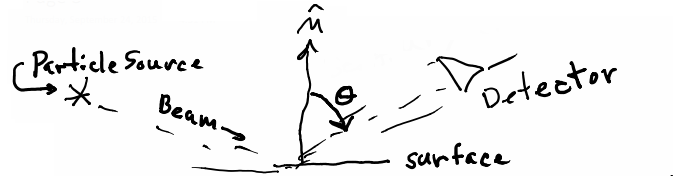
\includegraphics[height=080pt]{xrdDiffraction}
	\caption{Typical x-ray diffraction setup. The detector measures the beam intensity as a function of the scattered angle, $\theta$. The source, $\ast$, can be a photon, neutron, electron, molecule or other object.}
	\label{fig:xrd}
\end{figure}

The particles are not always diffracted. You can have a number of results for a given photon, including
\begin{enumerate}
	\item Absorption
	\item Exit particles
		\begin{enumerate}
			\item Flourescence
			\item Raman
			\item Scattered deflection
			\item Other
		\end{enumerate}
\end{enumerate}
\begin{figure}[h]
	\centering
	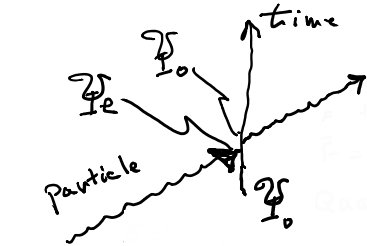
\includegraphics[height=60pt]{xrdDiffraction2}
	\caption{Quantum view of diffraction measurements. The system begins in a ground state $\Psi_0$. The particle causes an excitation to $\Psi_e$, which is followed by a relaxation to $\Psi_\text{new}$, which is oftened assumed to be $\Psi_0$.}
	\label{fig:quantumxrd}
\end{figure}
See Figure~\ref{fig:quantumxrd}. The initial energy of the system is:
\begin{align*}
	E &= \bar{h}\omega_\text{in}\\
	\vec{p} &= \bar{h}\vec{K}_\text{in}
\end{align*}

Upon relaxation, something comes out. As this happens, the system is likely to return to $\Psi_0$, and your particle continues with 
\begin{align*}
	E &= \bar{h}\omega_\text{scattering}\\
	\vec{p} &= \bar{h}\vec{K}_\text{scattering}
\end{align*}
\begin{subsection}{Energy}
	Balance of $E$\& $\vec{P}$
	\begin{align*}
		\bar{h}\omega_\text{in} &= \bar{h}\omega_\text{sys} + \bar{h}\omega_\text{scattered}\\
		\bar{h}\vec{K}_\text{in} &= \bar{h}\vec{q}_\text{sys} + \bar{h}\vec{q}_\text{scattered}\\
		\text{assume }\omega_\text{sys} &= 0\\
		\omega_\text{in} &= \omega_\text{scattered}
	\end{align*}
	Consider
	\begin{align*}
		\vec{K}_\text{in} - \vec{K}_\text{scattered} = \vec{q}_\text{sys}\\
	\end{align*}
	Since $\omega_\text{sys} = 0$, $\norm{\vec{k_\text{in}}} = \norm{\vec{q}}$
	\begin{align*}
		\vec{q} &= k(\hat{e}_\text{in} - \hat{e}_\text{scattered})\\
		k &= \frac{2\pi}{\lambda}
	\end{align*}
	This means that the incident and scattered particles have the \underline{same} energy. This is \underline{elastic} scattering.
	However, $\vec{q}_\text{sys}$ is \underline{not} zero but is determined by 
	\begin{align*}
		\vec{q}_\text{sys} = \vec{K}_\text{in} - \vec{K}_\text{scattered}
	\end{align*}
	However, since $W_\text{sys} = 0$,
	\begin{align*}
		|\vec{q}_\text{sys} | &= \sqrt{\vec{q}_\text{sys}\cdot \vec{q}_\text{sys}}\neq 0\\
		|\vec{q}_\text{sys} | &= | \vec{K}_\text{in} | = | \vec{K}_\text{scattered}|\\
		k &= \frac{2\pi}{\lambda}\\
		\vec{q}_\text{sys} &= k(\hat{e}_\text{in} - \hat{e}_\text{scattered})\\
		\vec{q} &= k(\hat{e}_\text{in} - \hat{e}_\text{scattered})
	\end{align*}

	\begin{figure}[h]
		\centering
		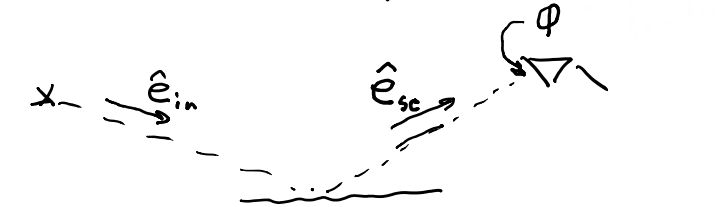
\includegraphics[height=60pt]{unitVectors}
		\caption{Diagram of the unit vectors. Note that $\phi$ is a field function. The detector is typically a square law detector. $\phi\ast\phi = i_\text{photocurrent}$, where $i_\text{photocurrent}$ is processed by electronics.}
		\label{fig:unitVectors}
	\end{figure}
	Light is thought of as a field, so this detector is seeing the field.

	Norm: $\sqrt{\vec{q}\cdot\vec{q}}$

	\begin{figure}[h]
		\centering
		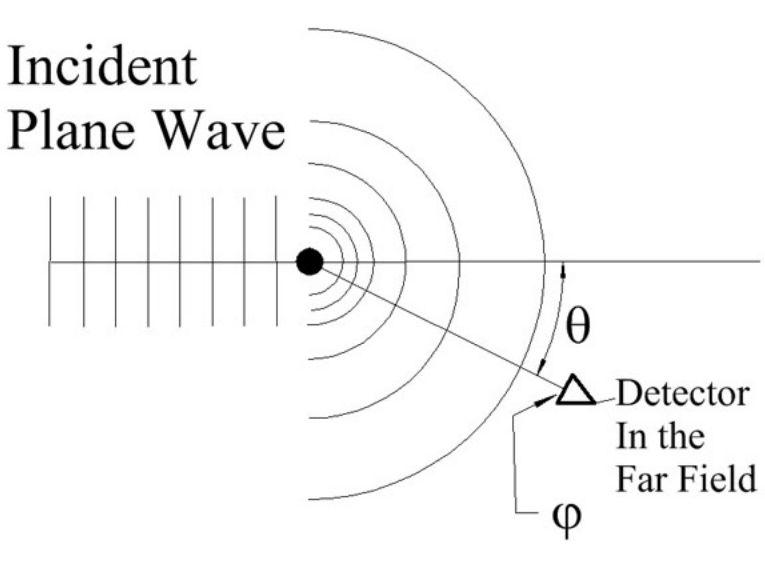
\includegraphics[height=80pt]{atomWave2}
		\caption{Look at diffraction from a small hole. Right at the detector level, we detect $\norm{\phi^2}$ for field $\phi$.}
		\label{fig:atomWave}
	\end{figure}


	\begin{align*}
		\vec{q} &= k(\hat{e}_\text{in} - \hat{e}_\text{scattered})\\
		\hat{e}_\text{in} &= (0,0,1)\\
		\hat{e}_\text{scattered} &= (\sin{\theta}\cos{\varphi},\sin{\theta}\sin{\varphi},\cos{\theta})
	\end{align*}
	If we take $\varphi=0$,
	\begin{align*}
		\vec{q} = k(-\sin{\theta},0,1-\cos{\theta})\\
		\sqrt{\vec{q}\cdot\vec{q}} = k\sqrt{2(1-\cos{\theta})}
	\end{align*}

	See if you can derive $q = \norm{\vec{q}}$ We will see how you did next time.

\end{subsection}
\begin{subsection}
	{Generating plane waves}
	\begin{figure}[h]
		\centering
		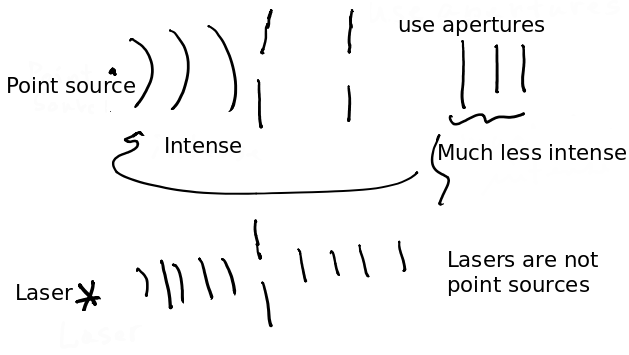
\includegraphics[height=120pt]{lasers}
		\caption{Diagram of point sources vs lasers}
		\label{fig:lasers}
	\end{figure}
	How to obtain plane waves: If you have a point source, you must use a lens-aperture system to obtain plane waves, which reduces the intensity of the wave. Lasers generate beams that are close to plane waves and they are intense. See Figure~\ref{fig:lasers}.
\end{subsection}
\begin{subsection}{Kinematic Approximation}
In the kinematic approximation
\begin{align*}
	\varphi = f_1 e^{i\vec{q}\cdot\vec{x}_1} 
\end{align*}
For particle $1$, $f_1$ is the scattering cross section.

In the kinematic approximation, you say for the set of particles:
\begin{align*}
	\varphi &= \sum_{n=0}^{N\times N} f_n e^{i \vec{q}\cdot\vec{x}_n}\\
	\vec{q} &= k(\hat{e}_\text{in} - \hat{e}_\text{scattered}
\end{align*}
$\phi$ is the electric field that is sampled by a square-law detector so that $\phi$ is ``converted'' to a current as $\phi\ast\phi$.
The E-field vector is $\vec{E} = \phi\hat{e}$, with $\hat{e}$ being a unit vector in some direction.

for the special case of a single kind of atom:
\begin{align*}
	f_n = f_m = f\\
	\therefore \frac{\phi}{f}\sum_{n=0}^{N\times N}e^{i\vec{q}\cdot\vec{x}_n}
\end{align*}
\begin{figure}[h]
	\centering
	\begin{subfigure}[t]{0.30\textwidth}
		\centering
		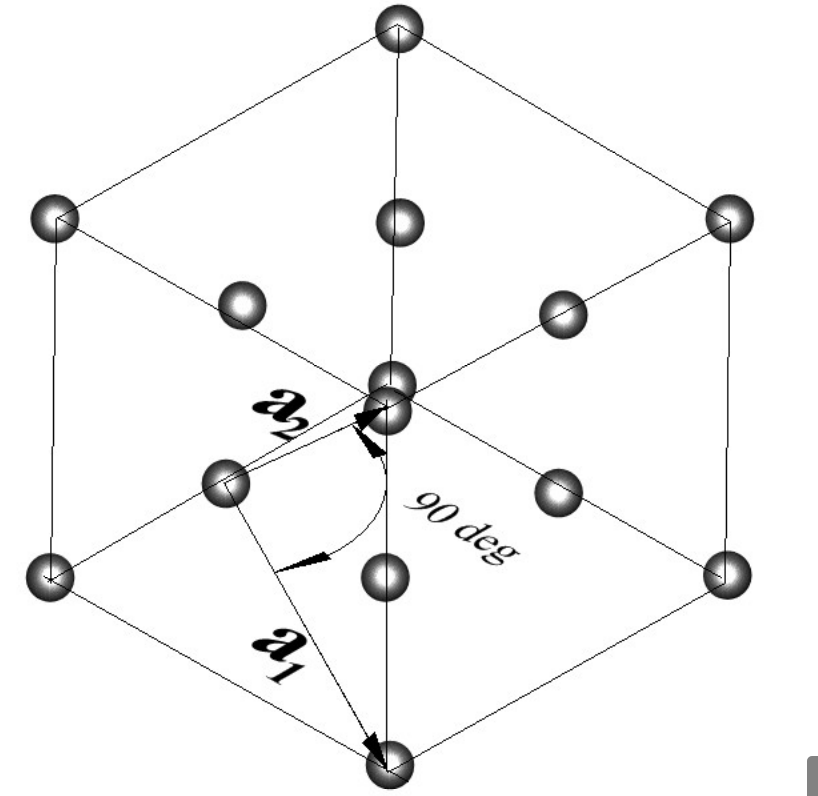
\includegraphics[height=60pt]{FCC100_2}
		\caption{FCC Crystal, such as Platinum}
		\label{fig:FCC}
	\end{subfigure}
	\begin{subfigure}[t]{0.30\textwidth}
		\centering
		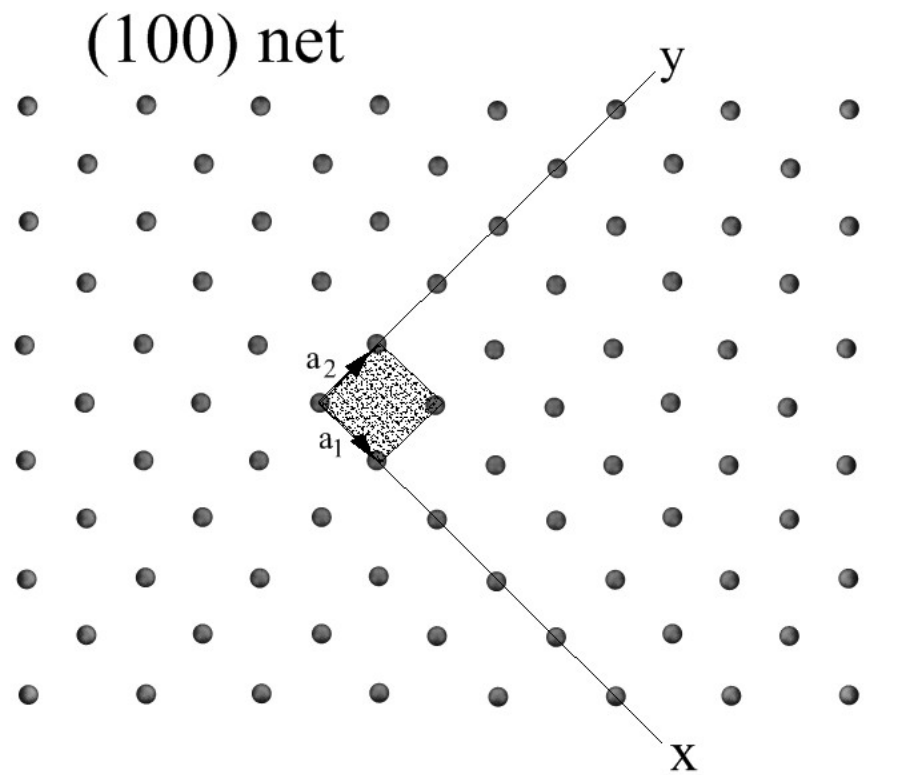
\includegraphics[height=60pt]{100plane2}
		\caption{2D lattice or net. This extends to the edge of the crystal.}
		\label{fig:Net}
	\end{subfigure}
	\begin{subfigure}[t]{0.33\textwidth}
		\centering
		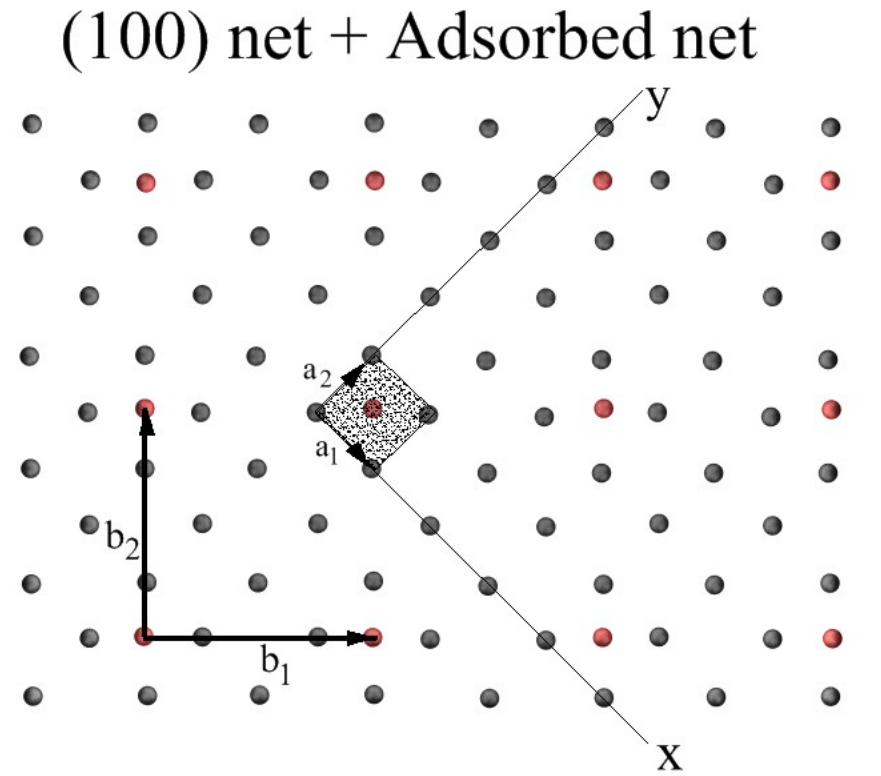
\includegraphics[height=60pt]{100plane2_ads}
		\caption{Net with adsorbed layer.}
		\label{fig:NetAds}
	\end{subfigure}
\end{figure}
Consider platinum for example. This one's important for lots of applications, it's an FCC crystal. The face may look something like Figure \ref{fig:FCC}
with atoms at each corner of the cube, with one in the center.  The angle between the center atom vectors is $90^\circ$. The plane shown is the (1 0 0) plane.

Suggest: If you've never done this, make sure that you see the geometry!

Figure~\ref{fig:Net} 
is a 2D lattice, known to surface chemists as a net. 

\note{You can get to any atom (atom at $\vec{x}_n$) by 
\begin{align*}
	\vec{x}_n = m_1 \vec{a}_1 + m_2\vec{a}_2
\end{align*}
where $m_1,m_2$ are integers $(0,\pm1,\pm2,\dots)$.}

Be sure that you see how that can be done. Construct a 1-to-1 map of $(m_1,m_2)$ to $\vec{x}_n$ as in Figure~\ref{fig:map}

\begin{figure}[h]
	\centering
	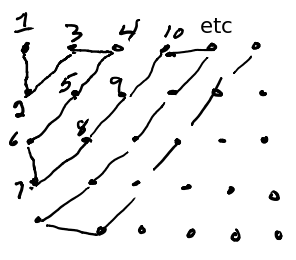
\includegraphics[height=80pt]{map}
	\caption{This construction tells you that $n$ is uniquely given by $\vec{x_n} = m_1 \vec{a}_1 + m_2\vec{a}_2$ when $\vec{a}_1$ and $\vec{a}_2$ are known.}
	\label{fig:map}
\end{figure}

What remains is to summarize the diffraction pattern.

You will find \begin{align*}\vec{x}_n = m_1\vec{a}_1 + m_2\vec{a}_2\end{align*} in diffraction space:
\begin{align*}
	\vec{q}_n &= h \vec{a}_1^\ast + k\vec{a}_2^\ast\\
	\vec{x}_n &\leftrightarrow \vec{q}_n
\end{align*}
This is the foundation of diffraction.

\note{
	\begin{itemize}
		\item	$\vec{x}_n$ is in direct space.
		\item $\vec{q}_n$ is in reciprocal space.
	\end{itemize}}\end{subsection}\end{section}
\begin{section}{References}
See Born \& Wolf ``Optics'', and Berne \& Pecora ``Dynamic Light Scattering'' for additional details about the electric fields.
\end{section}
\end{document}
